% Generated by code/scripts/report_figures.py at 2026-11-16T12:31:35Z; do not edit.
% Inputs: artifacts/cluster/runs/bench1-20261107T033925Z-1528774
\begin{figure}[t]
\centering
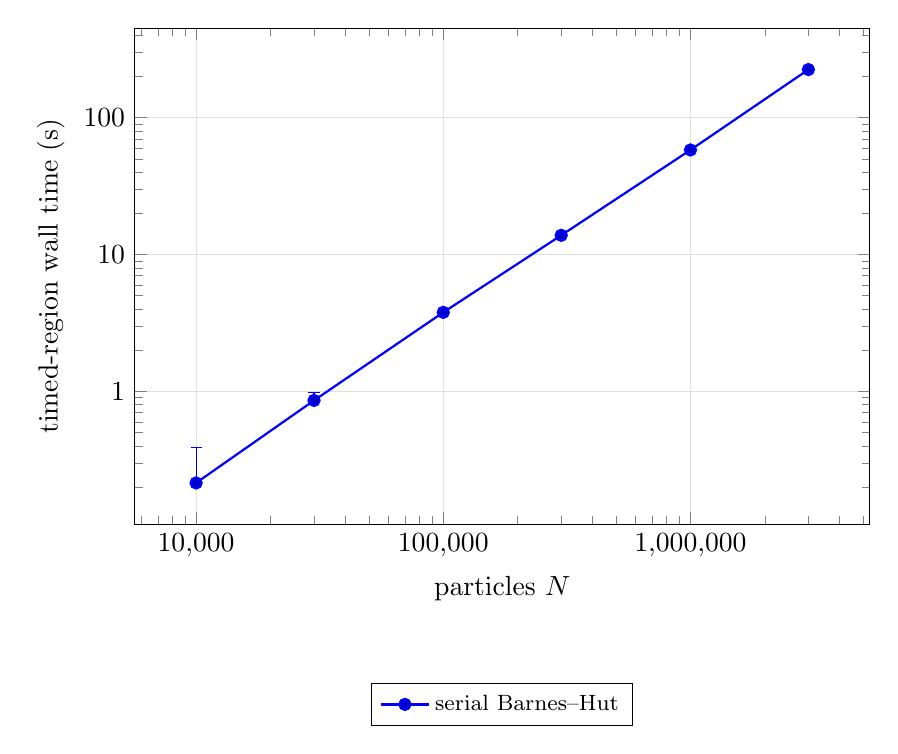
\begin{tikzpicture}
\begin{axis}[width=0.9\columnwidth, height=0.65\columnwidth, xlabel={particles $N$}, ylabel={timed-region wall time (s)}, xmode=log, log basis x=10, log ticks with fixed point, ymode=log, ytick={0.1,1,10,100,1000}, legend style={at={(0.5,-0.32)}, anchor=north, legend columns=2, font=\footnotesize}, legend cell align=left, grid=major, grid style={gray!25}]
\addplot+[mark=*, thick, error bars/.cd, y dir=both, y explicit] coordinates {(10000,0.2149) += (0,0.1727) -= (0,2.6e-05) (30000,0.8604) += (0,0.1236) -= (0,0.000664) (100000,3.784) += (0,0.002436) -= (0,0.001335) (300000,13.82) += (0,0.004285) -= (0,0.02243) (1e+06,58.05) += (0,0.1489) -= (0,0.04201) (3e+06,224.3) += (0,0.009573) -= (0,0.4536)};
\addlegendentry{serial Barnes--Hut}
\end{axis}
\end{tikzpicture}
\caption{Serial runtime against problem size, $\theta=0.5$, leaf size 8, 3 timed steps, median of repetitions. Least-squares slope on the log--log axes: 1.213. Bars: fastest to slowest repetition. Vanda job 1528774: all 64 cores of Gold 6438N node IN-008, 3 interleaved repetitions.}
\label{fig:serial-n}
\end{figure}
